The Large Hadron Collider (LHC) was created to explore the fundamental
properties of matter for the next decades.  Since LHC start-up in 2009,
multiple experiments  at LHC have collected and distributed hundreds of
petabytes of data worldwide to hundreds of computer centers. Thousands of
physicists analyze petascale data volumes daily. The detection of the Higgs
Boson speaks to the success of the detector and experiment design, as well as
the sophistication of computing systems devised to analyze the data.

Historically the computing systems consisted of the federation of a hundreds
to thousands of distributed resources \textemdash{} ranging in scale from
small to mid-size resource~\cite{foster2003grid}. Although the workloads to be
executed are independent, the management of the distribution of extremely-
large workloads across many heterogeneous resources to ensure the effective
utilization of resources and efficient execution of workloads presents non-
trivial challenges.

Many software solutions have been developed in response to these challenges.
One of the LHC experiments, the CMS experiment devised a solution based around
the HTCondor~\cite{XX} software ecosystem. The ATLAS~\cite{Aad:2008}
experiment, utilizes the Production and Distributed Analysis (PanDA) workload
management system~\cite{Maeno2011} (WMS) for distributed data processing and
analysis. The CMS and ATLAS experiments represent arguably the largest
production grade distributed computing solutions and have symbolized the
paradigm of {\it high-throughput computing} viz., the effective execution of
many independent workloads.

As the LHC prepares for the high-luminosity era (Run 3 in $~\approx$ 2022), it
is anticipated that the data volumes that will need analyzing will increase by
10X compared to the current phase (Run 2).   The data will be larger in volume
but will also require heterogeneous computational processes. In spite of the
impressive scale of the ATLAS distributed computing system, demand for
computing systems will significantly outstrip supply (availability).

There are multiple levels at which this problem needs to be addressed
urgently, e.g., the utilization of emerging parallel architectures (e.g.,
platforms), algorithmic and advances in analytical methods (e.g., use of
Machine Learning) and the ability to exploit different platforms (e.g., clouds
and supercomputers).

This paper is a case study of how the ATLAS experiment has "broken free" of
the traditional computational approach of high-throughput computing on
distributed resources to embrace new platforms, in particular high-performance
computers. Specifically, we discuss the experience of integrating the PanDA
workload management system with Titan ~\textemdash{} a DOE leadership
computing facility and scaled to analyze up to \jhanote{XX\%} of the ATLAS
experiment workload. We present the design of PanDA and show how localized
substitution to use well established pilot-concepts allow enhanced support for
heterogeneous workloads (such as molecular dynamics) and advanced execution
modes.

This state-of-practice paper provides multiple contributions.  (i) Documents
the many design and operational considerations that have been  taken to
support the sustained, scalable and production usage of Titan for historically
high-throughput workloads, (ii) Extensions to PanDA to support non-traditional
heterogeneous workloads and execution modes,  and (iii) As the community looks
forward to designing the next generation of online analytical platforms
~\cite{foap} the lessons learnt from our project provide some guidance for how
current and future experimental and observational systems can be integrated
with supercomputers in production.



% Historically, the ATLAS Computing model~\cite{jones2008atlas} is based on a
% Grid paradigm~\cite{foster2003grid}, with multilevel, hierarchically
% distributed computing and storage resources.

% PanDA has been developed to meet
% growing ATLAS production and analysis requirements for a data-driven workload
% management system capable of operating at LHC data processing scale.



% PanDA has a highly scalable architecture. Scalability has been demonstrated in
% ATLAS through the rapid increase in usage over the past several years of
% operations, and PanDA is expected to meet the continuously growing computing
% requirements of ATLAS over the next decade. PanDA was designed to have the
% flexibility to adapt to emerging computing technologies in processing, storage,
% networking as well as the underlying software stack. This flexibility has also
% been successfully demonstrated through the past six years: computing centers in
% ATLAS, spanning many continents, were seamlessly integrated into PanDA\@.

% PanDA manages a wide spectrum of workloads, ranging from raw data processing to
% Monte Carlo simulation and user analysis, while constantly evolving to meet
% rapidly changing science needs.

\mtnote{Used the following in related work. We may want to reduce/remove it from
the introduction: ``Today, PanDA serves several thousand users, managing job
distribution to hundreds of ATLAS sites with more than 100,000 CPU cores which
process more than a million jobs per day.''} % (Figure~\ref{fig:daily}).

% \begin{figure}
%     \begin{center}
%         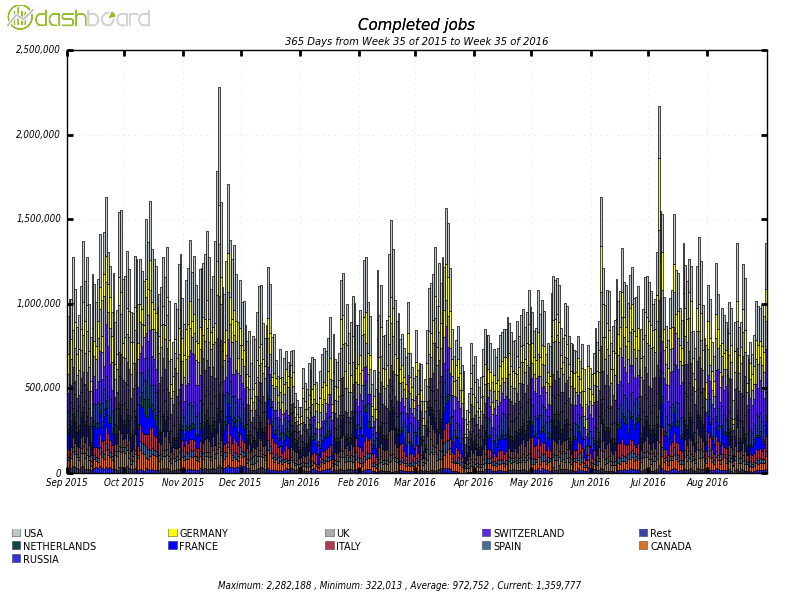
\includegraphics[width=\columnwidth]{figures/DailyJobs.png}
%         \caption{Daily completed jobs on ATLAS Grid for the past 12 month}
%     \end{center}
% \label{fig:daily}
% \end{figure}

In this paper, we describe how PanDA has been engineered to execute a specific
stage of the ATLAS Monte Carlo workflow on Titan, the larger high-performance
computing HPC system currently available in the USA\@.\mtnote{Explain the
benefits offered by Titan in terms of multithreading per node and possibly large
amount of concurrent nodes. Introduce also the notion of backfill.} This extends
the scope of PanDA's compute model, integrating both high-throughput and
high-performance computing resources and enabling the concurrent execution of
both  single and multi-core jobs. The integration of PanDA and Titan went
through three main engineering phases: (i) feasibility study and rapid
prototyping of an initial solution; (ii) progressing scaling of the  prototype
to saturate the available resources; (iii) study of a product-grade architecture
for generic HPC resources. Both phase i and ii have been completed enabling the
execution of up to eight million jobs a week on Titan. A prototype has been
engineered to support phase iii and experimental data are being collected.

In the next section we introduce \ldots.

Why Titan?
\begin{itemize}
    \item A lot of slow (relative the grid) and homogeneous cores together
    \item Grid is saturated
    \item Enable HPC as a calss of computing resource
    \item Enable future DOE experimental and observational capabilities on HPC
    \item Why is so important: more data, run 2 and run 3.
    \item growth of grid is flat (economic model) and saturated. We need more CPU because we have more data.
    \item ATLAS spend most of the time on simulations this is why we want to offload simulations - that happen happen to be performed via AthenaMP.
\end{itemize}





\subsubsection*{The following is a candidate for major compression into a single paragraph}


\mtnote{Moved from related work were we use already this terminology. To be
iterated/adjusted for consistency once the first draft will be ready.}

The term ``workflow'' is used in many disciplines with different meaning. In the
field of scientific computing, ``workflow'' assumes different meanings depending
on the characteristics of the computation, of the software tools used to support
this computation, and of the resources on which it is performed. Further, a
workflow may indicate a whole application, a description of the computational
process of that application or, more commonly, a series of tasks related by data
dependences.

The lack of a consistent and shared definition of ``workflow'' hinders the
understanding of its properties and its relations with related concepts. For
example, we need to clarify the difference among ``workflow'', ``workload'',
``task'', or ``job'' but also between workflow ``template'' and ``instance'', or
``data-flow'' and ``control-flow''. This is precondition to specify properly the
design of software systems that support the execution of scientific
applications.

In this paper, we use the following definitions:

\begin{description}

  \item[Task.] A set of operations to be performed on a computing platform,
  alongside a description of the properties and dependences of those operations,
  and indications on how the dependences should be satisfied and the operations
  should be executed.

  \item[Job.] A unit of  work performed by submitting a script to a resource
  management system (LRMS), like  Slurm or PBS, or by requesting a virtual
  machine or a container to a site supporting virtualization. One or more jobs
  can perform the operations described with a task.

  \item[Workload.] A set of jobs that can be executed concurrently, possibly
  related by a set of relations. For example, jobs of a workload can share one
  or more input files or communicate during execution.

  \item[Workflow.] Set of jobs, related by a set of relations that define the
  order in which each task can be executed. Data dependences are the most common
  relations among workloads, used to define the precedence among their
  executions.

\end{description}
